\section{Homology cross product}

In the last lecture we proved homotopy invariance of homology using the
construction of a chain level bilinear cross-product
\[
\times:S_p(X)\times S_q(Y)\to S_{p+q}(X\times Y)
\]
that satisfied the Leibniz formula
\[
d(a\times b)=(da)\times b+(-1)^pa\times(db)\,
\]
What else does this map give us? 

Let's abstract a little bit. Suppose we have three chain complexes $A_*$, $B_*$, and $C_*$, and suppose we have maps $\times: A_p\times B_q\to C_{p+q}$ that satisfy bilinearity and the Leibniz formula. What does this induce in homology?
\begin{lemma}
These data determine a bilinear map $\times:H_p(A)\times H_q(B)\to H_{p+q}(C)$.
\end{lemma}
\begin{proof}
Let $a\in Z_p(A)$ and $b\in Z_q(A)$. We want to define $[a]\times [b]\in H_{p+q}(C)$. We hope that $[a]\times [b]=[a\times b]$. We need to check that $a\times b$ is a cycle. By Leibniz, $d(a\times b)=da\times b+(-1)^pa\times db$. Because $a,b$ are boundaries, this is zero. Now we need to check that homology class depens only on the homology classes we started with.
So pick other cycles $a^\prime$ and $b^\prime$ in the same homology classes. We want $[a\times b]=[a^\prime\times b^\prime]$. In other words, we need to show that $a\times b$ differs from $a^\prime\times b^\prime$ by a boundary. We can write $a^\prime=a+d\overline{a}$ and $b^\prime=b+d\overline{b}$, and compute, using bilinearity:
	\begin{equation*}
	a^\prime\times b^\prime=(a+d\overline{a})+(b+d\overline{b})
	= a\times b+a\times d\overline{b} + (d\overline{a})\times b+(d\overline{a})\times(d\overline{b})
	\end{equation*}
We need to deal with the last three terms here. But since $da=0$,
\[
d(a\times\overline b)=(-1)^pa\times(d\overline b)\,.
\]
Since $d\overline b=0$, 
\[
d((\overline a)\times b)=(d\overline a)\times b\,.
\]
And since $d^2\overline b=0$, 
\[ 
d(a\times\overline{b})=
(d\overline a)\times(d\overline{b})\,.
\]
This means that $a'\times b'$ and $a\times b$ differ by 
\[
d\left((-1)^p(a\times \overline{b}) + \overline{a}\times b + \overline{a}\times d\overline{b}\right)\,,
\]
and so are homologous. 

The last step is to check bilinearity, which is left to the listener.
\end{proof}
This gives the following result.
\begin{theorem}
There is a map 
\[
\times:H_p(X)\times H_q(Y)\to H_{p+q}(X\times Y)
\]
that is natural, bilinear, and normalized. 
\end{theorem}

We will see that this map is also \emph{uniquely defined} by these conditions, unlike the chain-level cross product.

I just want to mention an explicit choice of $\iota_p\times\iota_q$. This is called the Eilenberg-Zilber chain. You're highly encouraged to think about this yourself. It comes from a triangulation of the prism. 

The simplices in this triangulation are indexed by order preserving injections
\[
\omega:[p+q]\to[p]\times[q]
\]
Injectivity forces $\omega(0)=(0,0)$ and $\omega(p+q)=(p,q)$. Each such map
determines an affine map $\Delta^{p+q}\to\Delta^p\times\Delta^q$ of the same name. These will be
the singular simplices making up $\iota_p\times\iota_q$. To specify the coefficients, think of $\omega$ as a staircase in the rectangle $[0,p]\times[0,q]$. 
Let $A(\omega)$ denote the area under that staircase. Then the Eilenberg-Zilber chain is given by 
\[
\iota_p\times\iota_q=\sum(-1)^{A(\omega)}\overline{\omega}
\]

\begin{center}
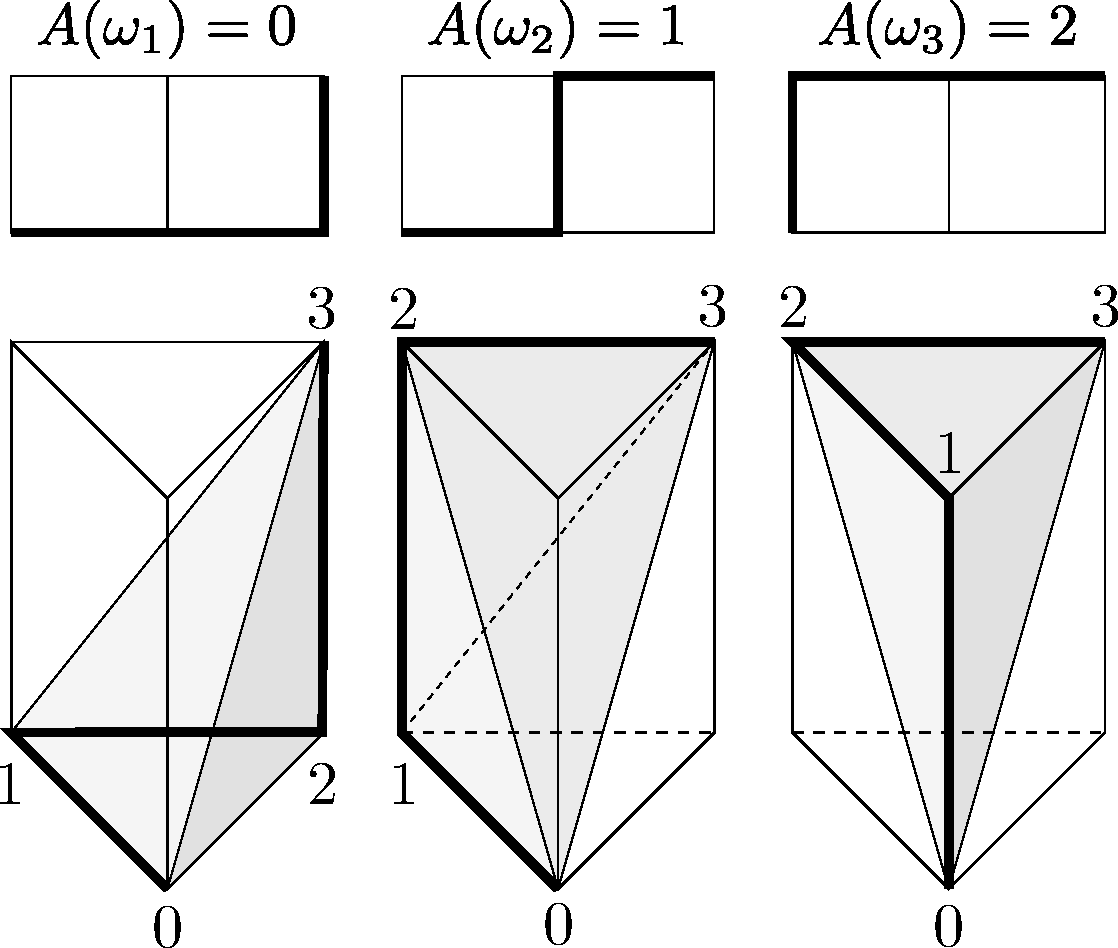
\includegraphics[width=5in]{905/Figures/07-EZ-triangulation.pdf}
\end{center}


This chain is due to Eilenberg and Mac Lane; the description appears 
in a paper \cite{eilenberg-moore} by Eilenberg and Moore. 
It's very pretty, but it's combinatorially annoying to check that this satisfies the conditions of the theorem. It provides an explicit chain map
\[
\beta_{X,Y}:S_*(X)\times S_*(Y)\to S_*(X\times Y)
\]
that satisfies many good properties on the nose and not just up to chain homotopy. For example, it's {\em associative} --
\[
\xymatrix{
S_*(X)\times S_*(Y)\times S_*(Z) \ar[r]^{\beta_{X,Y}\times 1} 
\ar[d]^{1\times\beta{Y,Z}} & 
S_*(X\times Y)\times S_*(Z) \ar[d]^{\beta_{X\times Y,Z}} \\
S_*(X)\times S_*(Y\times Z) \ar[r]^{\beta_{X,Y\times Z}} &
S_*(X\times Y\times Z)
}\]
commutes -- and {\em commutative} --
\[
\xymatrix{
S_*(X)\times S_*(Y) \ar[r]^{\beta_{X,Y}} \ar[d]^{T} & 
S_*(X\times Y) \ar[d]^{S_*(T)} \\
S_*(Y)\times S_*(X) \ar[r]^{\beta_{Y,X}} \ar[r] & S_*(X\times Y)
}\]
commutes, where on spaces $T(x,y)=(y,x)$, and on chain complexes
$T(a,b)=(-1)^{pq}(b,a)$ when $a$ has degree $p$ and $b$ has degree $q$. 

We will see that these properties hold up to chain homotopy for any 
choice of chain-level cross product.

